
\newpage

\section{Models}

\subsection{Introduction}
A model is the single, definitive source of information about one’s data. It contains the essential fields and behaviors of the data one is storing. Generally, each model maps to a single database table. The Models module manages the data, logic and rules of the database.


\subsection{Schema}
Apart from the User Model, mentioned in the Social Auth Module, the major entities of the application are, Problem, Contest, Participant, Submission, Tag and Post.
\begin{figure}[h!]
    \centering
    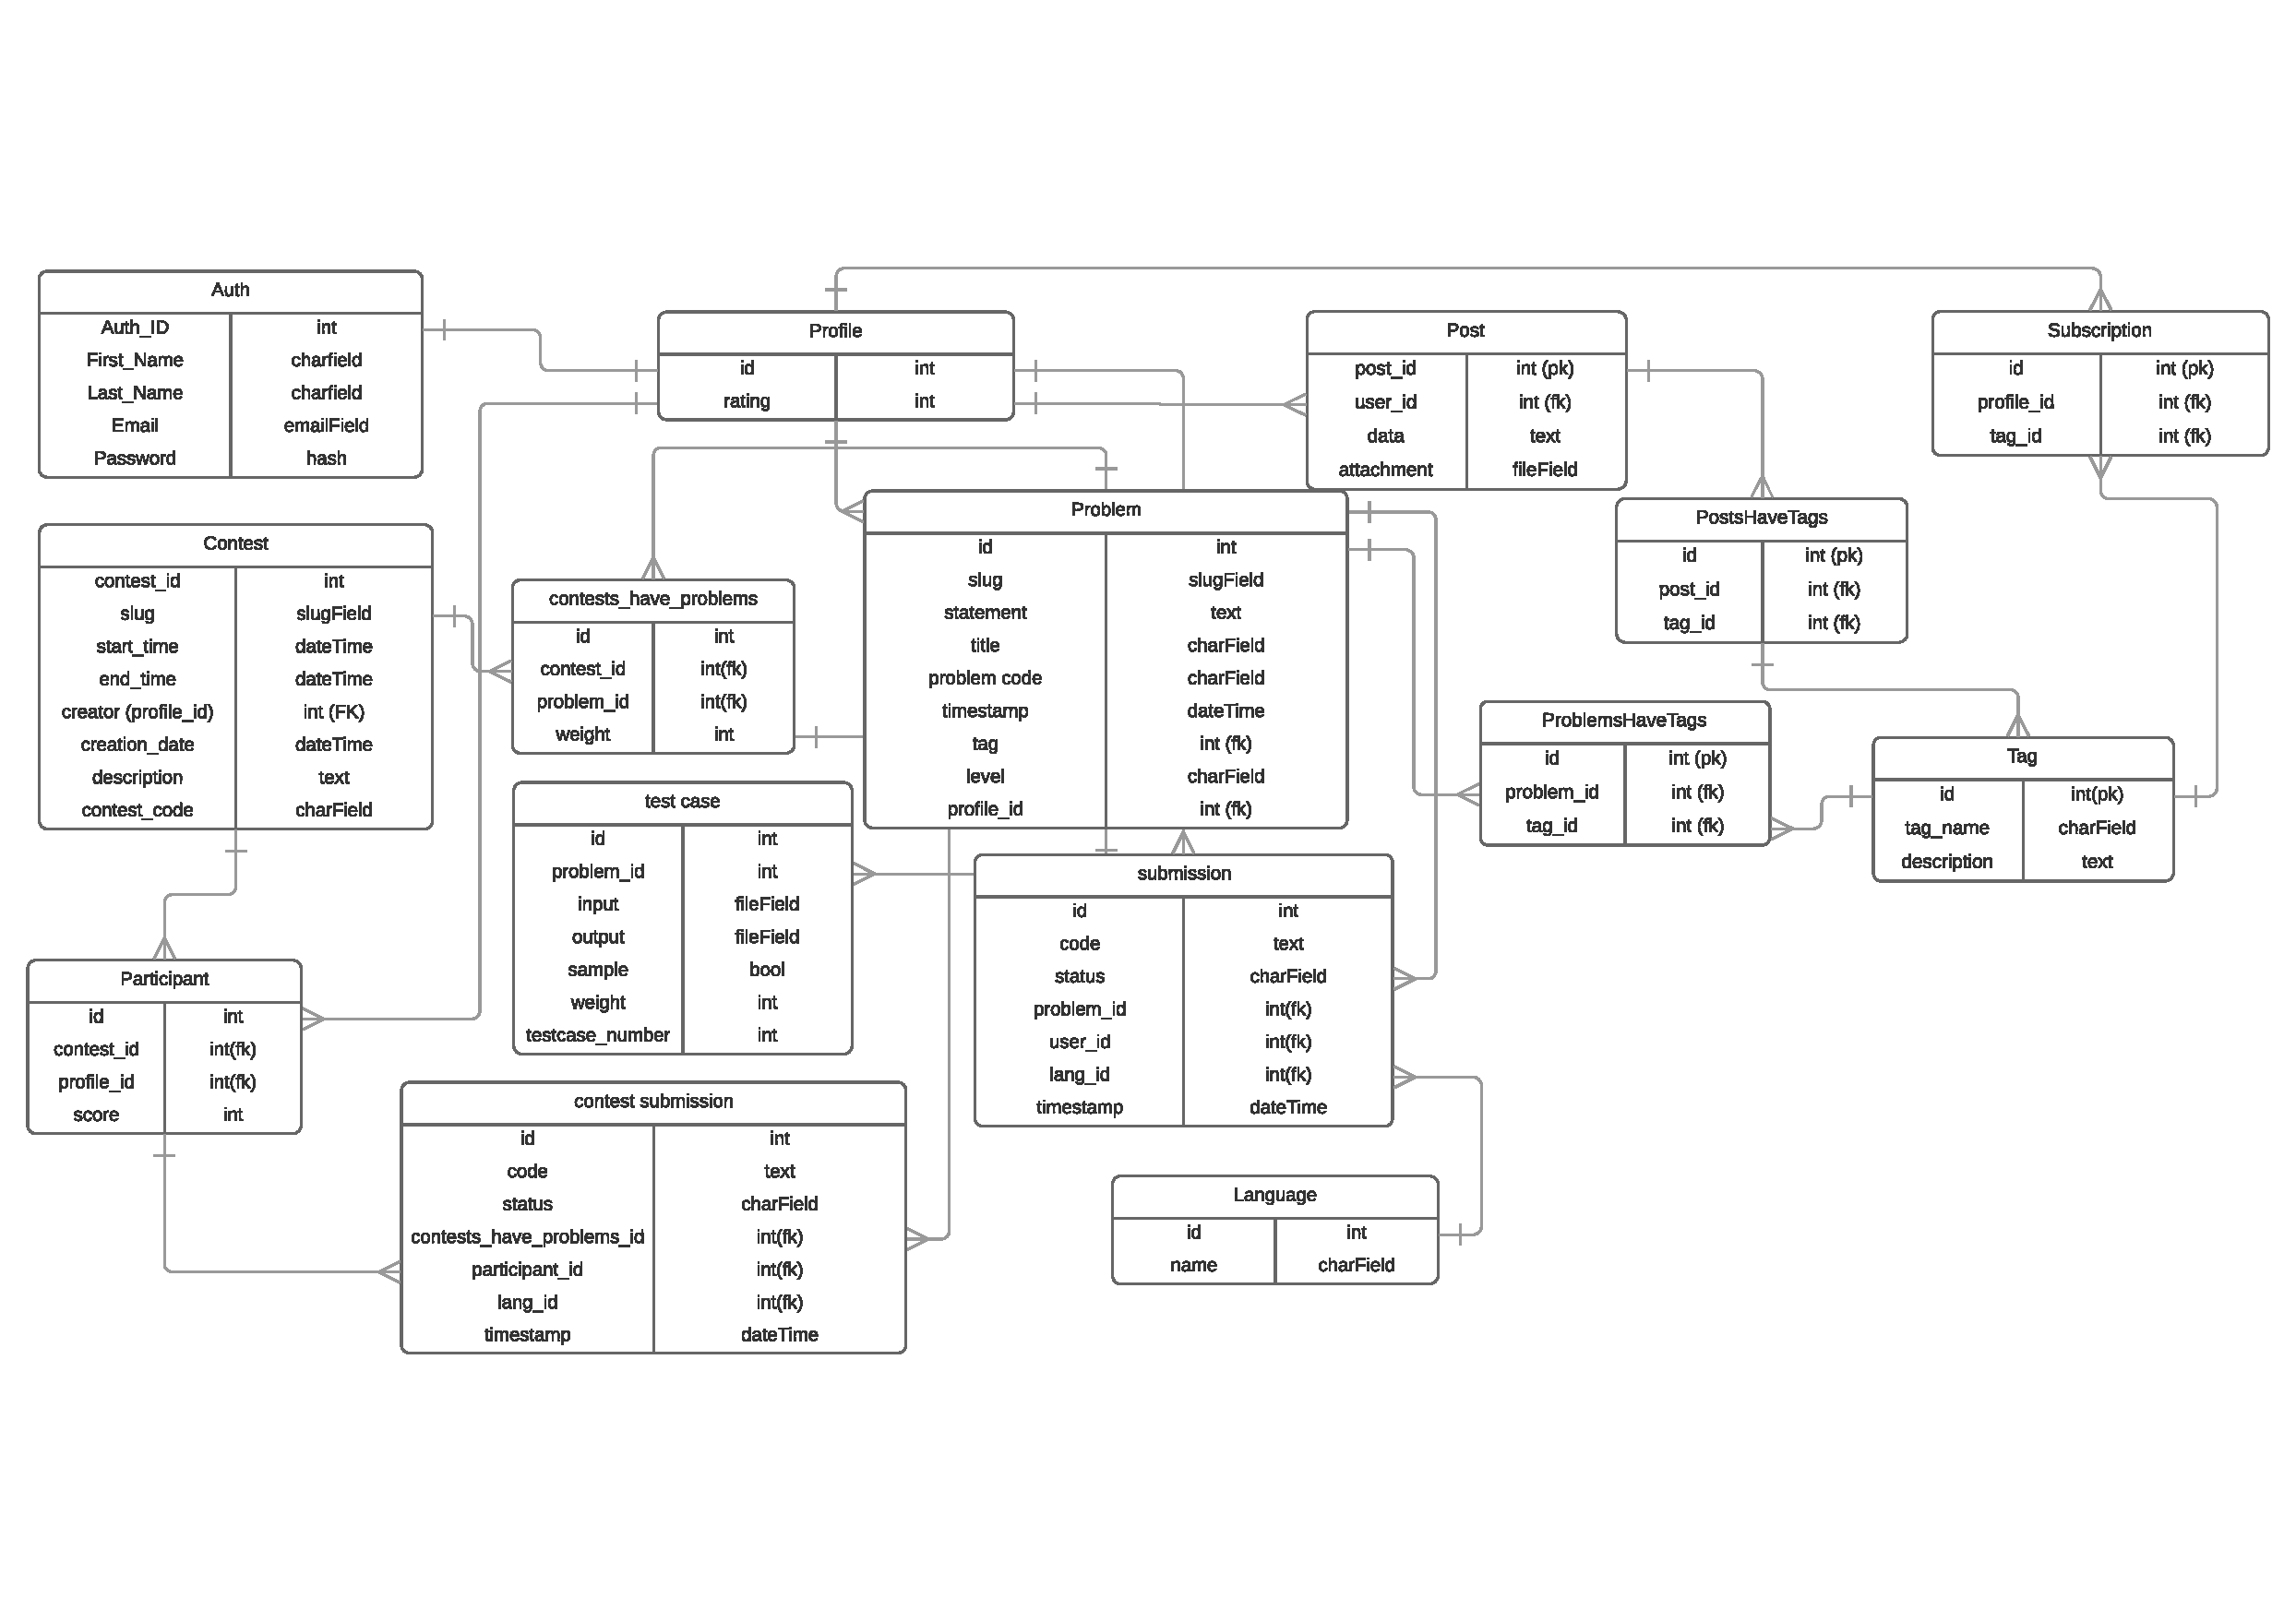
\includegraphics[width=\linewidth]{modules/schema.pdf}
    \caption{ER Diagram}
    \label{fig:schema}
\end{figure}

\vspace{1cm}

\subsubsection{Problem}
Consisting of a title, problem statement, level of difficulty, problem setter and test cases, the problem model represents a problem in the application. The model has a one-many relationship with Test Case, a many-one relationship with User and a many-many relationship with Contest. The model also contains problem code, which is a unique code given to the problem, as well as a slug field which is derived from the problem code. A slug field is used to store and generate valid URLs for dynamically created web pages. 

A \textit{pre\_save signal}, a signal (set of instructions) sent before the instance of a model is saved in the database, is used to generate a slug from the problem code.

\subsubsection{Test Case}
Consisting of an input file, an output file, test case number and weight, the Test Case Model represents a test case of a problem. The test case number attribute stores the value of the test case and the weight attribute representing the weight that specific test case has in the problem. There is a boolean attribute sample, which checks whether the test case is a sample test case.

The input and output files are stored in a folder named with the unique problem code, having names $<$test case number$>$.in and $<$test case number$>$.out, respectively.

\subsubsection{Contest}
Consisting of a title, description, starting time, ending time, and contest creator, the contest model represents a contest in the application. The model has a many-one relationship with User (creator of the contest), a many-many relationship with Problem and a many-many relationship with User (participants of the contest). The model also contains contest code, which is a unique code given to the problem, as well as a slug field, similar to the one in the Problem Model, which is derived from the problem code. 

\subsubsection{Contest Problem}
The many-many relationship between the Problem and Contest model is through the model Contest Problem, which represents a problem in the contest. Apart from foreign keys from both the models, it has a weight attribute representing the weight that specific problem has in the Contest.

\subsubsection{Participant}
The many-many relationship between the User and Contest model is through the model Participant, which represents a participant in a contest. Apart from foreign keys from both the models, it has a score attribute representing the total score of the user in the contest.

\subsubsection{Submission}
Consisting of a submitter, code, language, problem and status, the submission model represents a user submission. A user submission is sent to the Judge Module to get back the status of the submission. The current languages supported and status options are mentioned in the judge module.

\subsection{Future Plans}
Outside the contest environment, the application aims to extend its functionality by introducing two new models, Post and Tag, if time permits.

\subsubsection{Post}
Consisting of a title, description, optional attachment and creator, the post model represents a post. A post might be an article about some algorithm or some latest updates in the world of computer science. Various posts can be seen by a user on their homepage.

\subsubsection{Tag}
A tag is helpful in filtering out various posts and problems for a user. It has a many-many relationship with Post and Problem. Users can subscribe to specific tags to get updates on their feed.